
% Chapter X

\chapter{The importance of genome assembly} % Chapter title

\label{ch:01-03} % For referencing the chapter elsewhere, use \autoref{ch:name} 

%----------------------------------------------------------------------------------------
Most of the genomic techniques presented earlier cannot be performed without having a high quality sequence of the genome of the species investigated at hand. Ideally, a complete reference would consists to a telomere-to-telomere genome, as downstream analyses will rely on the relative positions of different biological elements on the genome sequence to draw biological conclusions. 

The availability of several sequenced genomes closely related to the species of interest is also crucial for comparative analyses. This allows for example to identify \acrshort{HGT} events, perform comparative genomics analysis, and investigate the evolution of molecular processes. However, for many species, full reference genomes remain incomplete or nonexistent. Several worldwide efforts have been undertaken to generate catalogs of the genomes of all existing species, broadening the number of species with their full genome being sequenced. Until recently, the only eukaryotic genomes with telomere-to-telomere sequences, and (almost) no gaps within the chromosomes, consisted in fungi with compact genomes species such as \textit{Saccharomyces cerevisiae} or \textit{Schizosaccharomyces pombe}, the worm \textit{Caenorhabditis elegans} \cite{yoshimuraRecompletingCaenorhabditisElegans2019,mewesOverviewYeastGenome1997}. Here we describe in more detail the process of genome assembly and its relevance to infection genomics.

\section{From reads to chromosomes}
% Define terminology, explain advantages of chromosome level assemblies and how to generate them
% Subsections for bionano, linked reads and Hi-C
% Maybe a quick mention of haplotype-resolved assemblies and genome-graphs

Genome assembly consists in reconstructing the linear sequence of the genome from the readings of DNA by different sequencing technologies. Although the final assembly depends on the quality of these readings, the algorithms used to combine their information are also crucial.

%  First viruses, then yeast
In the early days of genome sequencing, the Sanger and Gilbert methods were used to read DNA sequences \cite{sangerDNASequencingChainterminating1977,maxamNewMethodSequencing1977}.These are low throughput, but highly accurate sequencing methods. These technologies allowed to unveil the complete genome sequences of viruses \citep{sangerNucleotideSequenceBacteriophage1982,baerDNASequenceExpression1984,vanwezenbeekNucleotideSequenceFilamentous1980} followed by chromosome III of \textit{S. cerevisiae}, the first eukaryotic chromosome to be sequenced \cite{oliverCompleteDNASequence1992}. A common practice at the time, was to clone small genomic regions of \textasciitilde 10-30 kb into a plasmid resulting in a bacterial artificial chromosome, amplify it in bacteria and extract it \cite{thierryCompleteSequenceKb1990}. The positions of those clones and relative order on the chromosome were then determined by digesting them into restriction fragments and hybridizing them to identify overlaps and construct a physical map of the chromosome \cite{mcphersonPhysicalMapHuman2001}. Each clone was then randomly fragmented and sequenced. The sequencing readout, in the form of gels, had to be deciphered by scientists, one nucleotide at a time. The cloned region was then assembled manually by searching for overlaps between fragments.

Further technological improvements allowed to automate the sequencing process to tackle the sequencing of larger eukaryotic genomes. Early genome sequencing projects were performed using laborious and costly experimental methods, such as \acrfull{BAC}, which involved cloning long overlapping pieces of DNA of the genome into bacteria. These pieces were then experimentally amplified and sequenced in parallel. Overlapping ends from each of those sequences had to be aligned to recover the entire chromosome sequence. The first genome sequencing projects were sizable undertakings requiring the collaboration of many research groups throughout the world \citep{collinsNewFiveyearPlan1993,adamsGenomeSequenceDrosophila2000,oliverCompleteDNASequence1992}, but technological advancements progressively reduced the cost and time required. A decisive change was the development of shotgun sequencing \cite{venterSequenceHumanGenome2001}, which involves randomly sequencing regions to cover the entire genome.

With the advent of \acrfull{NGS}, shotgun sequencing became the standard for whole genome sequencing. \acrshort{NGS} has much higher throughput than Sanger sequencing, allowing to sequence megabases of DNA very quickly. However, it can only read short sequences at a time, referred to as \Gls{read}s. Classic overlap-based genome assembly algorithms used in previous sequencing projects could not scale to such large numbers of short reads. This called for the development of more efficient genome assembly algorithms.

The goal of an assembler is to generate a highly contiguous genome sequence from a large number of short reads. Early algorithms computed pairwise alignments between all reads to build an overlap graph (Fig. \ref{fig:01-03:debruijn}a). The genome could then be assembled by finding the Hamiltonian path of the graph, which passes once through every node. However, finding this approach is computationally expensive and cannot be used with high sequencing throughput \cite{compeauHowApplyBruijn2011}. This lead to the development of de Bruijn-based assembly algorithms, which many modern assemblers still use \citep{simpsonABySSParallelAssembler2009,zerbinoVelvetAlgorithmsNovo2008}. de Bruijn assemblers split reads into short \Gls{k-mer}s which they use to generate a de Bruijn graph. In these graphs, k-mer sequences represent edges, and the overlap between adjacent k-mers within reads are the nodes (Fig. \ref{fig:01-03:debruijn}b). To assemble a genome, assemblers need to find the Eulerian path, which passes through every edge once. However this is often not possible because of repeated sequences in the genome, sequencing errors and haplotypes \cite{simpsonTheoryPracticeGenome2015}. Whenever a repeated sequence is longer than the read itself, the graph can not be solved and heuristics have to be used. Rather than a single fully resolved genome, the resulting assemblies usually have a relatively high number of independent pieces called \Gls{contig}s.

\begin{figure}
\centering
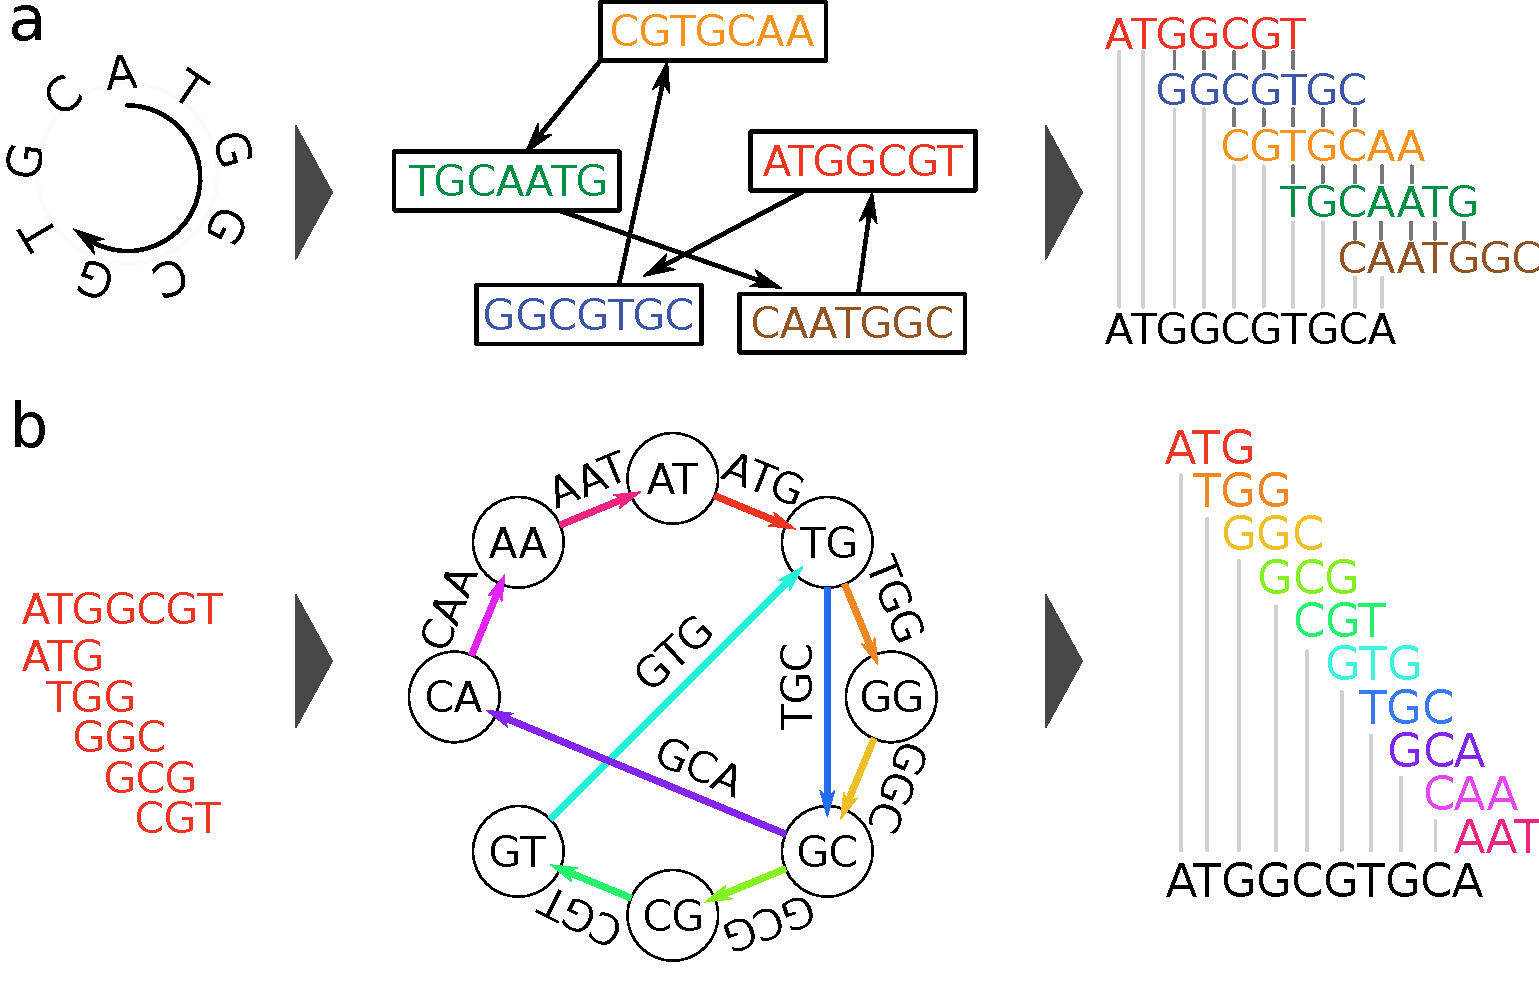
\includegraphics[width=0.85\textwidth]{Parts/Part01/gfx/debruijn.pdf}
\caption[Graphs in genome assembly.]{Graphs in genome assembly: A small circular genome is sequenced and the resulting reads are shown in color \textbf{a}: Early assembling techniques computed all pairwise alignments between reads to represent them as nodes in an overlap graph and their overlaps as edges. The genome sequence can be retrieved by finding a path going through each read exactly once. \textbf{b}: Modern assemblers first split reads into their constituent k-mers and represent the k-mers as edges in a de Bruijn graph where nodes are the k-1 overlap between two k-mers located in the same read. The path going through each edge once is computed to solve the graph. K-mers are extracted from the edges visited to retrieve the genome sequence. Adapted from \cite{compeauHowApplyBruijn2011}}
\label{fig:01-03:debruijn}
\end{figure}12

Third generation sequencing partially alleviates this issue by generating long albeit less accurate reads. Read lengths up to hundreds of thousands of basepairs can be generated, which allows to span most repeated regions. Recently, these technologies were used to generate telomere-to-telomere assemblies of several human chromosomes \citep{migaTelomeretotelomereAssemblyComplete2020,logsdonStructureFunctionEvolution2021}. Third generation sequencing techniques still suffer from their lower base calling accuracy resulting in assemblies with high point error rates (>10\%) and indels \cite{weiratherComprehensiveComparisonPacific2017,jainNanoporeSequencingAssembly2018}. To remove these errors, some methods have been developed to correct long reads before assembly, either by correcting long reads among themselves \cite{morisseScalableLongRead2021}, or using a separate set of short accurate reads to erase sequencing errors in long reads \cite{wangFMLRCHybridLong2018}. Most long reads correction tools are also unable to differentiate between SNPs and sequencing errors, which result in the loss of haplotype information and prevents the generation of haplotype-resolved assemblies. Some long read correction methods have recently been developed to preserve haplotypes information \cite{holleyRatatoskHybridError2021}. One major drawback of read correction methods is their high computational cost, as they require to align high number of reads to each other. An alternative strategy is to use the uncorrected reads to assemble the genome and perform error correction directly on the assembly, a process known as \Gls{polishing}. Traditional short read polishers work by aligning short reads to the assembly and replacing each position of the assembly by the consensus of short reads \cite{vaserFastAccurateNovo2017}. Additionally, they can correct larger scale misassemblies such as indels by using the pair-end information and alignment discrepancies \cite{walkerPilonIntegratedTool2014}. Some polishers have obtained better polishing accuracy by combining the information in short and long reads \cite{kunduHyPoSuperFast2019}.

%% ROMAIN STOPPED HERE %%%

The last sequencing technology in date is the HiFi platform from Pacific Biosciences which allows fairly long (10-25kb) but very accurate (<1\% error rates) reads, thus offering a comfortable middle ground between Nanopore and Illumina reads \cite{wengerAccurateCircularConsensus2019}. This trade-off has made HiFi reads popular for genome assembly \cite{langComparisonTwoUptodate2020,chengHaplotyperesolvedNovoAssembly2021,chengHaplotyperesolvedNovoAssembly2021}. Their low error rates have also enabled algorithmic developments with drastically lower computational costs for the assembly of large metagenomes \cite{ekimMinimizerspaceBruijnGraphs2021}.

Recently, the emergence of specialized technologies aimed at scaffolding have allowed to generate even more continuous and correct genomes at reduced costs. One example is the recent rebirth of optical mapping to introduce fluorescent probes into chromosomes at specific sites \cite{lamGenomeMappingNanochannel2012}. The order of these probes and their relative distance form barcodes which can then be used to scaffold genome assemblies, reorder and merge contigs. This is often combined with Hi-C to generate highly continuous assemblies even in the presence of repeated sequences.

A growing number of genome assemblies combine several of these different technologies to bring the number of scaffolds as close as possible to the real number of chromosomes (Fig. \ref{fig:01-03:assembly}).

\begin{figure}[htb]
    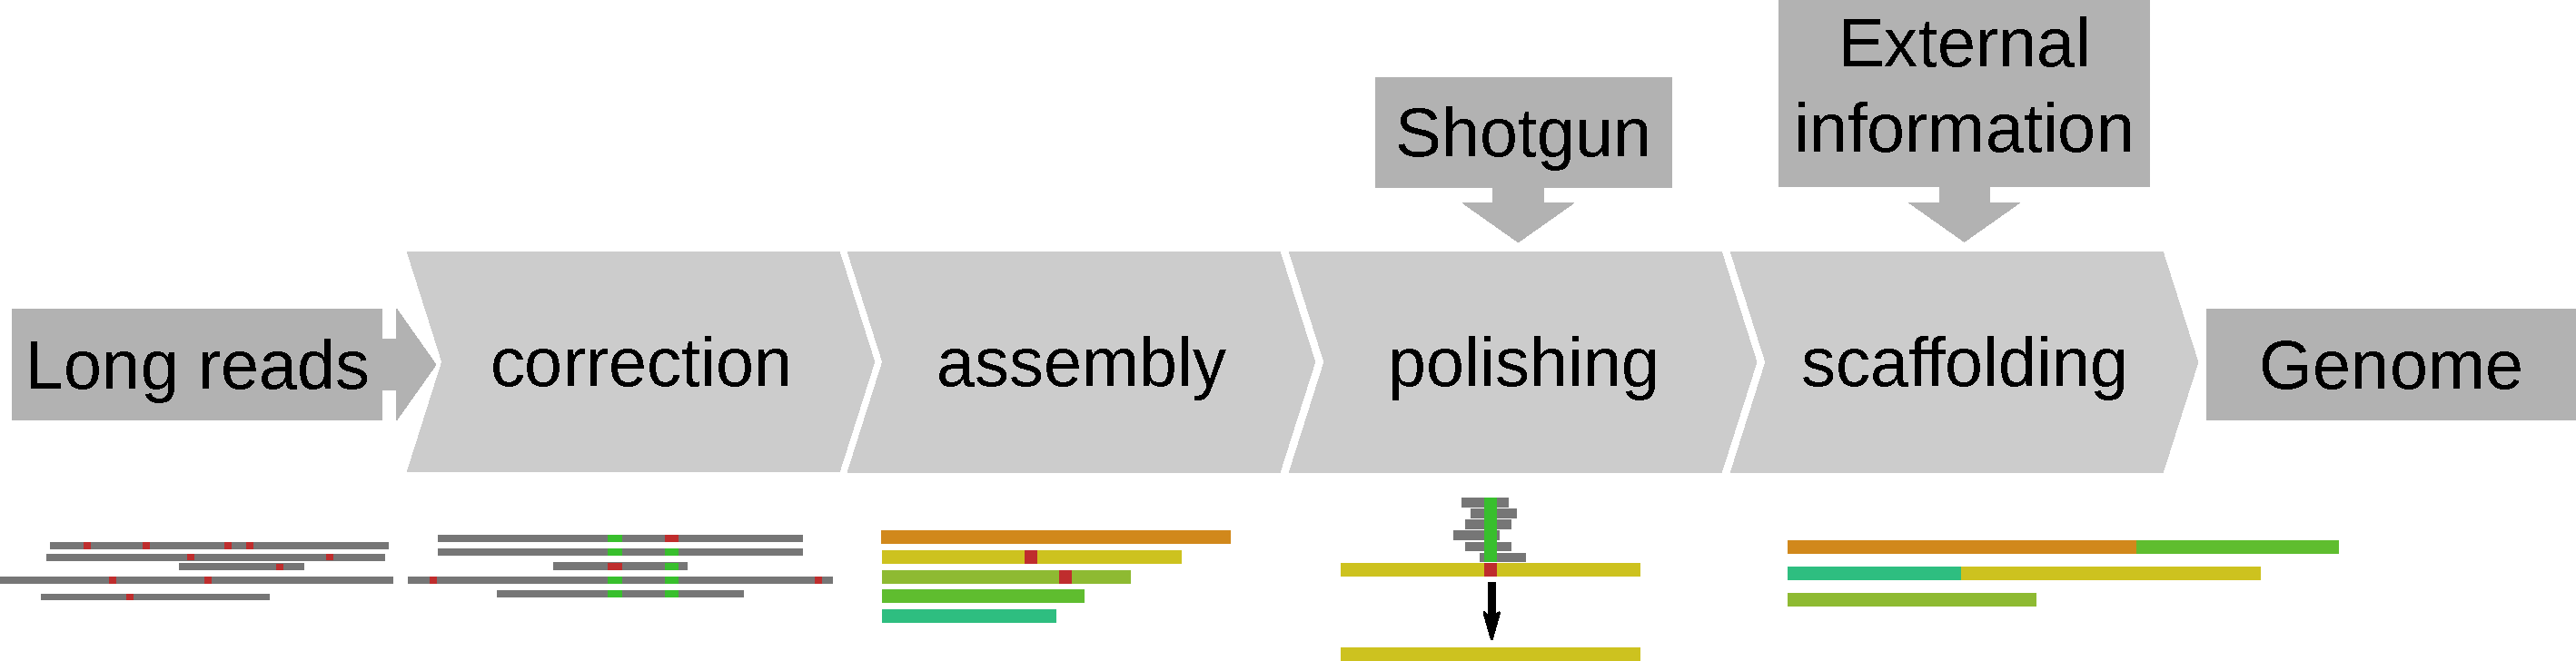
\includegraphics[width=\textwidth]{Parts/Part01/gfx/assembly_pipeline.pdf}
    \caption[Example of a third generation sequencing assembly pipeline.]{Example of a typical assembly pipeline using third generation sequencing. The error prone long reads are first corrected by pairwise comparisons. The corrected reads are assembled into contigs using their overlaps. The remaining sequencing errors in the assembly are removed by polishing with accurate short reads. Other sources of information can then be used to combine contigs into scaffolds.}
    \label{fig:01-03:assembly}
\end{figure}

\section{Phylogenetic representation}
% HGT detection requires a reference group

A common way to analyse the genome of new microorganisms is to compare it to other species. To achieve this, one needs to have other closely related genomes available. A common case where dense species genome representation is required is when attempting to detect \acrshort{HGT}.

\acrshort{HGT} detection methods often rely on discordance between gene trees and species trees. A horizontally transferred gene between two distant species would show strong sequence similarity \cite{ravenhallInferringHorizontalGene2015}. For this reason, detection of recent events requires genomes of closely related organisms as a comparison point.

\begin{figure}[htb]
    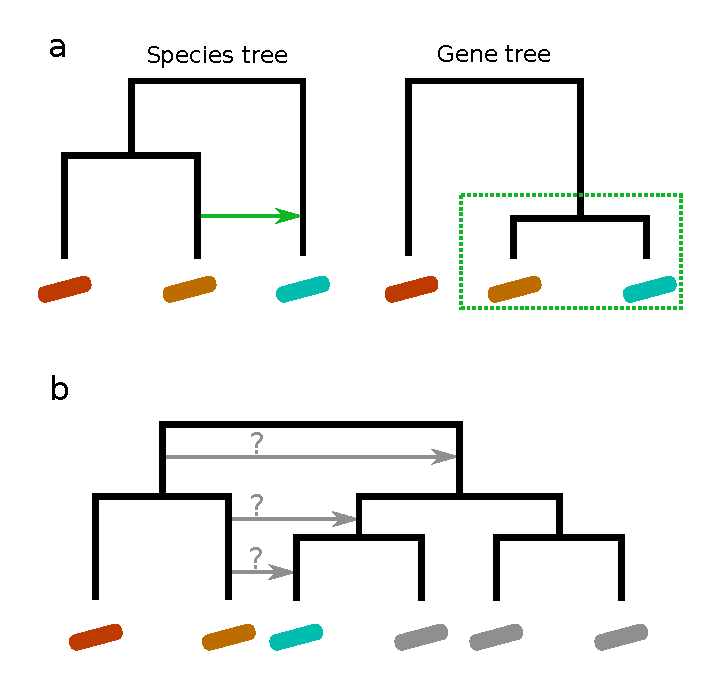
\includegraphics[width=\textwidth]{Parts/Part01/gfx/phylo_hgt.pdf}
    \caption[Phylogenetic representation of an HGT event.]{Phylogenetic representation of an HGT event. \textbf{a:} An HGT event between two species (shown with a green arrow) can be detected through discrepencies between the species (left) and gene (right) trees. \textbf{b:} In cases where genomes of closely related species are unavailable (greyed out organisms), the origin of the horizontal transfer cannot be accurately inferred (possible events shown with grey arrows).}
    \label{fig:01-03:phylo-hgt}
\end{figure}

Another frequent analysis when comparing a group of strains or species of microorganisms is to define the set of genes they contain, known as pangenome. This also allows the identification of genes specific to a  subset of these genomes, known as accessory genome. Such sets can be helpful to determine metabolic reactions associated with species or niches, however they heavily depend on the proportion of available species in the group.

Lately, several large consortia \citep{genome10kcommunityofscientistsGenome10KProposal2009,poelchauI5kWorkspaceNAL2015,DarwinTreeLife} undertook the daunting task of sequencing thousands of organisms throughout the tree of life. For the aforementioned reasons, these large collaborations are likely to greatly improve the power of comparative genomic analyses results in the future.

\section{The transition to genome graphs}

Until recently, all reference genomes were exclusively stored as linear (or circular) sequences of DNA. This linear sequence is often obtained from a mix of multiple individuals, or alleles within an individual. It is effectively a semi-arbitrary combination of multiple haplotypes collapsed into an artificial consensus sequence. A more accurate alternative is to produce a reference sequence graph instead \cite{churchExtendingReferenceAssembly2015}. Given a collection of haplotypes, individuals, or strains of a species, one can generate a graph where identical regions are collapsed, while sample-specific variants form bubbles retaining the genetic variability. As this approach is relatively recent, few algorithms have been developed to operate on sequence graphs, making their applications very limited.

The shift to genome graphs is promising for the analysis of bacterial samples, where alignment can be performed on multiple strain references at the same time. Doing this with a collection of linear genomes incurs mapping bias due to ambiguous alignments of redundant regions between references \cite{liDesignConstructionReference2020}. Similarly, genome graphs also allow systematic alignment to different alleles in polyploid organisms, solving the issue of allele-specific mapping bias in linear references \cite{vandegeijnWASPAllelespecificSoftware2015}. 
